\documentclass{article}
\usepackage{csvsimple}
\usepackage[margin= 1in]{geometry}
\usepackage{graphicx}
\graphicspath{ {Documents/desarrollo_overview} }
\begin{document}
   \begin{center}
      \Large\textbf{Neurodesarrollo Overview}\\
      \large\textit{Sarah M. Quander} \\
      \large{August 16, 2016}
   \end{center}

\section{General Overview}
Modelo Integral para el Desarrollo Infantil Temprano (MIDIT) is a program implemented in Mexico by Un Kilo de Aydua to push Early Childhood Development to the forefront of Mexican legislation. The central mission of Un Kilo de Aydua is to eradicate child malnutrition in Mexico by the year 2024. The interventions performed by MIDIT sought to generate impactful economic and social return and provide key insight into the importance of Early Childhood development when developing a nation. MIDIT was implemented through 3 programs: Physical Development, Neurodevelopment/Psychoaffective, and Community Development. Through the implementation of these 3 programs Un Kilo de Ayda performed holistic assessments of children's conditions and were able to develop comprehensive treatments tailored to the community. 

\subsection{Physical Development Program}
The Physical Development Program was the first program implemented by UKA. The program was developed in 2000 and entailed UKA distributing nutritional packets to participants. Bi-Monthly, the program would record the weight and height of the subject to track the development of the children once they were given nutritional supplements and foods. In 2002 the program also began recording hemoglobin levels of participants to help treat and identify participants which have anemia. The Physical Development Program has four core components:
\begin{itemize}
\item Food and Nutrition: Improve the nutritional status of children under 5
\item Breastfeeding: Increase the prevalence of breastfeeding 
\item Maternal and Preventative Health: Reduce morbidity/mortality in children from diarrheal and respiratory diseases
\item Supplementation and Micronutrients: Prevent and correct micronutrient deficiencies  
\end{itemize}
\subsection{ Neurodevelopment/Psychoaffective Program}
The Neurodevelopmental program was initiated in 2008 and aims to ensure the proper emotional environments through ensuring the following two components:
\begin{itemize}
\item Timely Stimulation: ensure that children under five experience sufficient daily stimulation.
\item Parenting Practices: ensure parents take the necessary steps to develop the emotional and affective abilities of children.
\end{itemize}
\subsection{ Community Development Program}
Community development is an essential factor in ensuring longterm success in Early Childhood Programs. In 2003 the program began implementing workshops to provide valuable schooling to children and educational classes for adults. In  2010 water sanitation programs were initiated to ensure the communities had access to sanitized and hygienic water. In the MIDIT program, favorable environments were self-sufficiently produced through ensuring:
\begin{itemize}
\item Food Security: Communities have access to locally produced, nutritionally sufficient, and preferable foods which are fiscally accessible to all members of the community.
\item Water and Sanitation: Communities have access to water which satisfies human, productive, and environmental needs.
\item Access to Basic Services: Communities have access to education, health, and housing services which improve the quality of live of children in the community. 
\end{itemize}
To ensure the effectivity of the this program MIDIT adopted three strategies to ensure maximum engagement of the community. MIDIT utilized Huertos Integrales Demostrativos (HID), which were public spaces where community members could take classes, participate, and help build housing, education centers, and health centers. The Centro Integral Demostrativo (CID) is a space where classrooms can be build with the help of UKA and the community. Finally,  Huertos Integrales de Traspatio (HIT) are replicas of the HID space but located in the individual community members home. These three spaces each are meant to engage the community such that they feel a personal investment in the program.

\section{Geography}
The state, municipal, and local town for each subject is recorded along with numeric ID's associated with each of the aforementioned. In total there are 9 states, 661 municipalities, and 1,827 towns represented within the data. The 9 states include: Chiapas, Estado de Mexico, Guerrero, Oaxaca, Puebla, San Luis Potosi, Sinaloa, Veracruz, and Yucatan. The altitude of each subjects home was recorded, a description of these altitudes are depicted in the table below.
\begin{center}
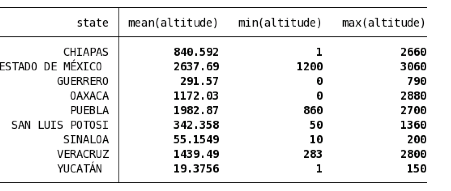
\includegraphics[scale=.75]{altitude}

\end{center}

\section{Population}
Over the span of 14 years, 267,993 children participated in the MIDIT programs. Each subject was assigned to one of 32 test centers, where they were additionally each assigened to a test proctor for the duration of their participation in the program. On average each subject participated in the program for 16 months, with the minimum recorded duration being 1 day, and the the maximum recorded duration being 170 months. Subjects who did participate in the program for a prolonged period of time visited the test center bi-monthy, thus on average each participant has 8 recorded visits to their respective test center. The name and date of birth of each subject is recorded along with the assigned identification number of the participant. The gender breakdown is relatively balanced. Of the 367,993 observations, 51.31 percent are male and 48.69 percent are female. 188,822 of the subjects identify as male and 179,171 subjects identify as female. 
\begin{center}
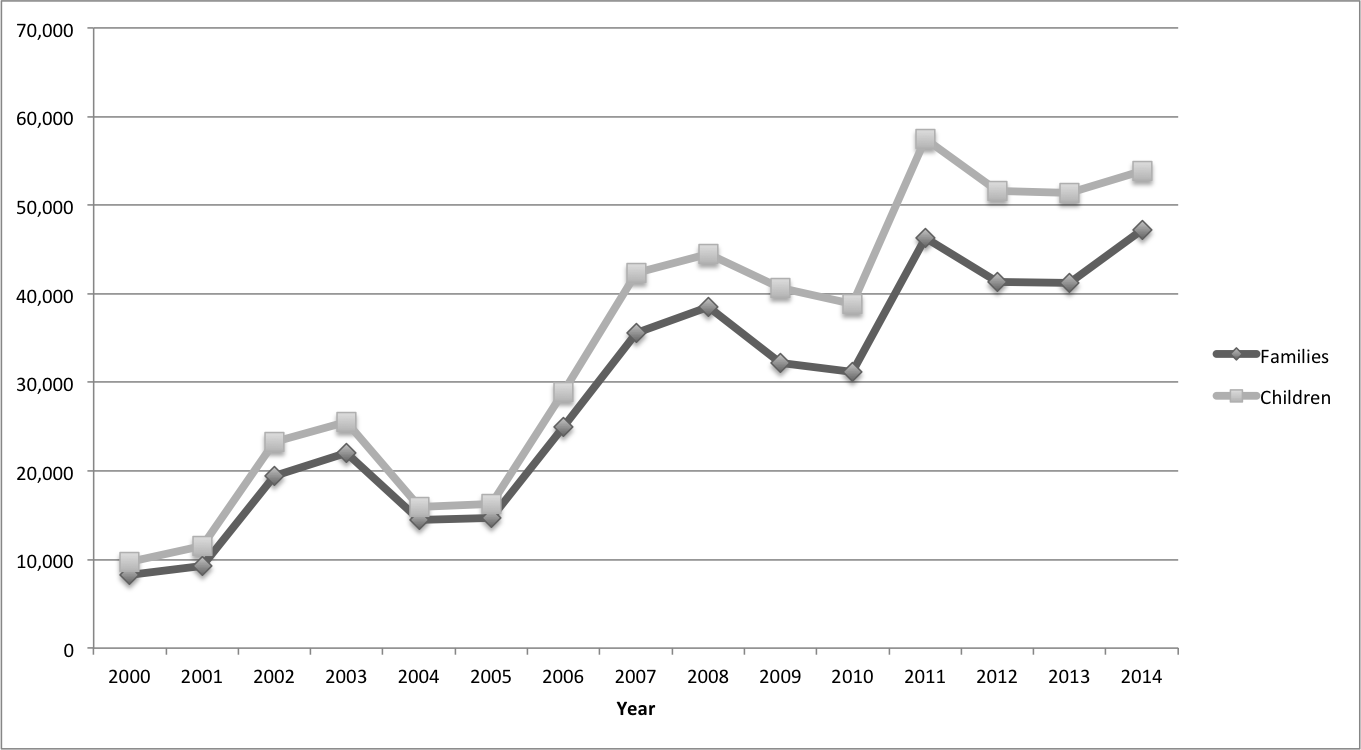
\includegraphics[scale=.5]{children.png}
\end{center}
The target participants in the program were children under the age of 5. It is in this age range which UKA felt they could impement the largest long-lasting impacts on the subjects lives. The average initial age of the children is 23.43157 months with a standard deviation of 25.5 months and the average final age is 36.02482 months with a standard deviation of 27.03 months.  


\begin{figure}[!htb]\centering
   \begin{minipage}{0.49\textwidth}
     \frame{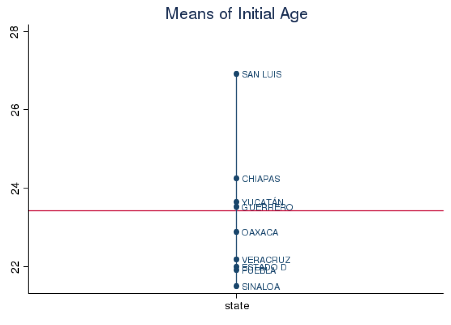
\includegraphics[width=\linewidth]{age_initial}}
   \end{minipage}
   \begin {minipage}{0.49\textwidth}
     \frame{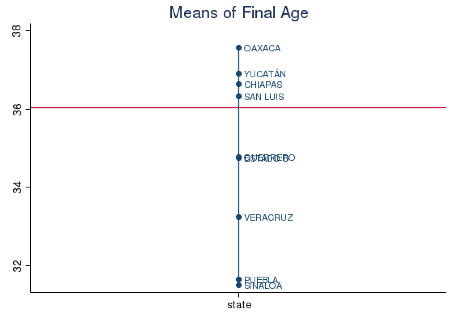
\includegraphics[width=\linewidth]{age_final}}
   \end{minipage}
\end{figure}

\section{Test Measures}
Variables recorded include weight, age, height, HB levels, and Anemia levels. The weight of the subjects was measured in kilograms the variable which was most consistently recorded. Height variables were also recorded consistently and were measured using centimeters. Both of these variables were recorded bi-monthly. Additionally there are variables which record the date of each weight and height measurement and the age of the individual at the time of the measurement. The zscore of the participant and a string variable clearly states the participant as either underweight, normal, overweight, or obese are also recorded and derive from the original height and weight values.

\begin{center}
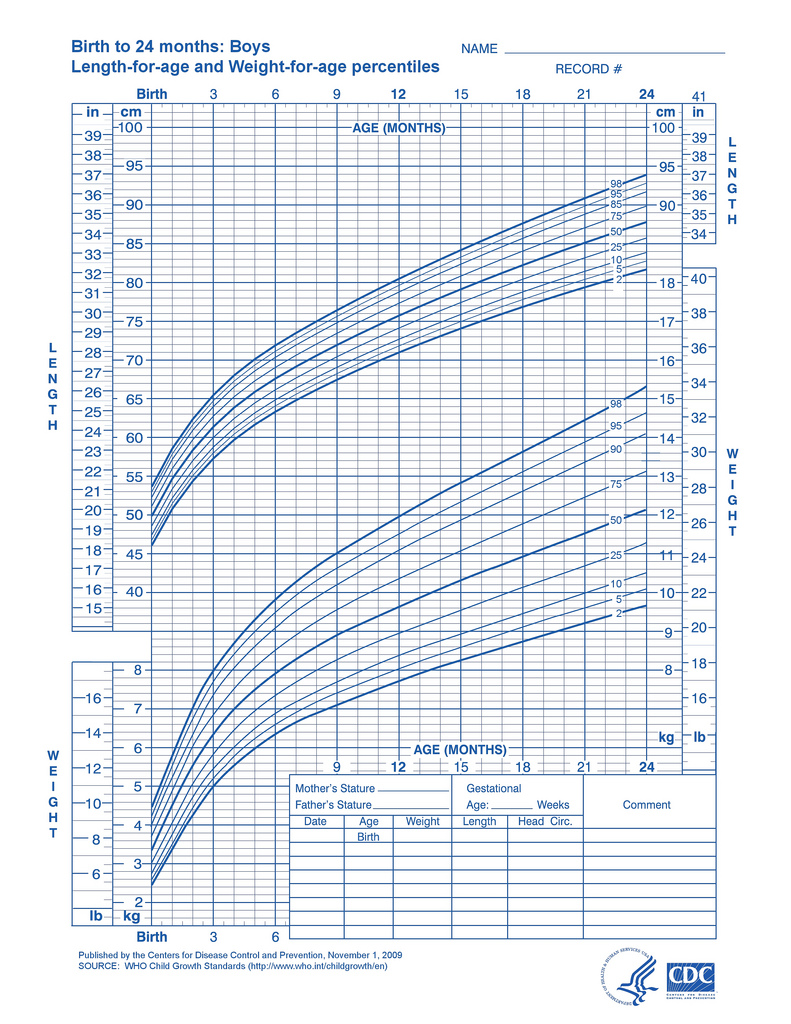
\includegraphics[width=100mm]{weight_length_babies.jpg}
\end{center}

As aforementioned, in 2002 the program began to identify and treat anemia. Participants were identified has having anemia though measurement of their hemoglobin blood levels. Normal results for newborn is between 14-21 g/dL while normal levels for infants is between 9.5-13 g/dL; as the subject ages the normal ranges will increase again until they are an adult. For adults the normal range of hemoglobin levels is between 12.1 and 17.2 g/dL. In the data a binary system is used to indicate if the subject has anemia; a '1' indicates the subject has normal hemoglobin levels while a '2' indicates the subject is anemic. 

\section{Program Growth}
The MIDIT programs began in 2000 with 6 test centers spread across 4 states: Chiapas, Estado de Mexico, Oaxaca, and Yucatan. Over the course of the next 14 years the program expanded as depicted below.
\begin{center}
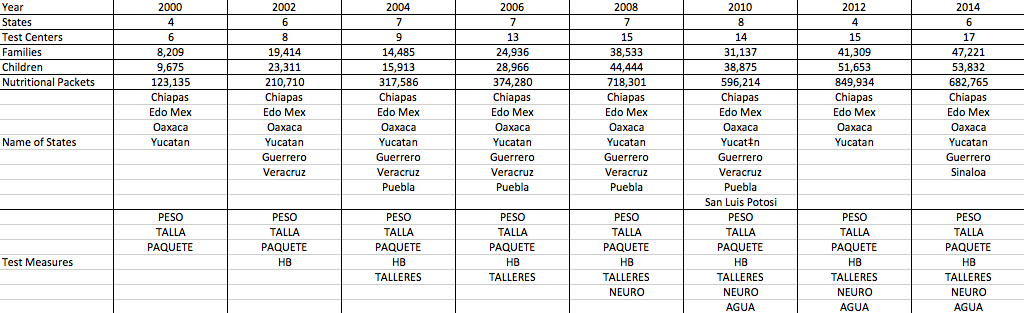
\includegraphics[scale=.51]{growth}
\end{center}




\end{document}